\documentclass{standalone}
\usepackage[x11names]{xcolor}
\usepackage{tikz}
\usetikzlibrary{shapes,arrows,decorations.markings, arrows.meta}
\usetikzlibrary {positioning}
\usetikzlibrary{calc}
\usetikzlibrary{patterns}
\usepackage{enumitem}
\usepackage{helvet}
\usepackage[T1]{fontenc}

%---------------------------------- Colors
\definecolor{color0}{RGB}{228,26,28}
\definecolor{color1}{RGB}{55,126,184}
\definecolor{color2}{RGB}{77,175,74}
\definecolor{color3}{RGB}{152,78,163}
\definecolor{color4}{RGB}{255,127,0}
\definecolor{color5}{RGB}{255,255,51}
\definecolor{color6}{RGB}{166,86,40}
\definecolor{color7}{RGB}{247,129,191}
\definecolor{color8}{RGB}{153,153,153}
\definecolor{color9}{RGB}{0,0,0}

\tikzstyle{simpleNode} = [rectangle, draw, fill=color0, text width=2cm, text centered, minimum height=2cm]

%----------------------------------------------------------------------------------
\def \nodeDistance {2.8cm}


\begin{document}
	\nopagecolor
	
	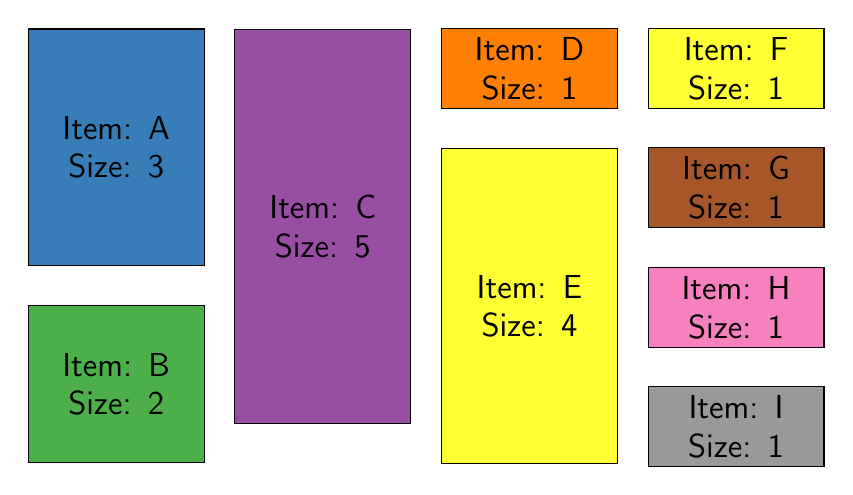
\begin{tikzpicture}[node distance = 2cm, auto,font=\sffamily\large]
	
	\node[simpleNode, minimum height=3cm, fill=color1](Item-A){Item: A\\Size: 3};
	
	\node[simpleNode, minimum height=2cm, fill=color2]at([yshift=-1.5cm]Item-A.south)(Item-B){Item: B\\Size: 2};
	
	\node[simpleNode, minimum height=5cm, fill=color3]at([xshift=1.5cm, yshift=0.5cm]Item-A.south east)(Item-C){Item: C\\Size: 5};
	
	\node[simpleNode, minimum height=1cm, fill=color4]at([xshift=1.5cm, yshift=-0.5cm]Item-C.north east)(Item-D){Item: D\\Size: 1};
	
	
	\node[simpleNode, minimum height=4cm, fill=color5]at([yshift=-2.5cm]Item-D.south)(Item-E){Item: E\\Size: 4};
	
	
	\node[simpleNode, minimum height=1cm, fill=color5]at([xshift=1.5cm]Item-D.east)(Item-F){Item: F\\Size: 1};
	
	\node[simpleNode, minimum height=1cm, fill=color6]at([yshift=-1cm]Item-F.south)(Item-G){Item: G\\Size: 1};
	
	\node[simpleNode, minimum height=1cm, fill=color7]at([yshift=-1cm]Item-G.south)(Item-H){Item: H\\Size: 1};
	
	\node[simpleNode, minimum height=1cm, fill=color8]at([yshift=-1cm]Item-H.south)(Item-I){Item: I\\Size: 1};

	\end{tikzpicture}
\end{document}